%\documentclass[10pt]{beamer}

\documentclass[handout]{beamer}
\usepackage{pgfpages}
\pgfpagesuselayout{6 on 1}[a4paper,border shrink=0mm]

\usepackage{amsmath,amssymb,longtable,hhline}
\usepackage{mathrsfs}
\usepackage{xcolor}
\usepackage{hyperref}
\usepackage{multicol}
\usepackage{anyfontsize}
\usepackage{minted}
\usepackage{alltt}
\usepackage{tabularray}

%\usepackage{pgfpages}
%\mode<handout>{\setbeamercolor{background canvas}{bg=white}}
%\pgfpagesuselayout{8 on 1}[a4paper,border shrink=2mm]
%\pgfpagesuselayout{2 on 1}[letterpaper,border shrink=2mm]


%%%%%%%%%%%%%%%%%%%%%%%%%%%%%%%%%%%%%%%%%%%%%%%%%%%%%%%%%%%%%%%%%%%%%%%%%%
% Первопорядковый логический вывод при решении задач распознавания с использованием результатов, полученных алгоритмически и нейросетевыми методами

% Кривовато, конечно.....  Погуглил, я так понял в России этим вообще никто не занимается сейчас.

% План доклада:
% 1. Модель управления из книги С.Н.Васильева, 2000 (Интеллектное управление динамическими системами).
% 2. Достижение современных методов на нейронных сетях (классифицирующие сети, синтезирующие сети).
%     Проблема автоматической оценки соответствия результата требованиям (у нейронок).
% 3. Проблематика распознавания характеристик динамических систем и сценариев (что-то не могу найти классическую литературу о них, будто бы мне приснилось). В сценариях нас интересуют параметры (т.е. модель с т.з.  исследования параметров, не forecasting).
% 4. Предлагаемая архитектура и инструментарий на основе объектно-ориентированного языка Logtalk.
% 5. Примеры: Синтез библиотеки визуальных классов Rapidminer для ППП Mothur,
%     Распознавание структуры рабочих программ вузов (PDF->Структура текста),
%     (новая задача) Распознавание береговой линии водохранилищ по спутниковым снимкам с использованием универсального сегментатора изображения Segment Anything (он только сегментирует изображения, но не дает им features, порождает только маски, но делает он это очень хорошо) совместно с данными Openstreetmap (семантической ГИС-разметки). Тут, правда мы на пол пути еще, но ... задача интересная.
% 6. В Заключении говорим о двух вещах.
%     6.1. Можно время тратить на подготовку данных для обучения, обучение и тестирование Нейронных сетей. Проблема с качественным обучением - вычислительные ресурсы.
%     6.2. Боремся с фундаментальной проблемой соответствия результата НС (нейросеть) требованиям - создаем инструмент контроля непротиворечивости результатов нейронных сетей "внутри" правил систем, основанных на формализованных знаниях. Т.е. если данные с НС формируют "удачное" соответствие секции "если" правил, то результаты можно считать близкими к истине. Это типа перекрестного допроса.
%%%%%%%%%%%%%%%%%%%%%%%%%%%%%%%%%%%%%%%%%%%%%%%%%%%%%%%%%%%%%%%%%%%%%%%%%%%%%%%



\usemintedstyle{tango}
\newcommand{\ltprgsize}{\fontsize{5}{5}\selectfont}
%\newcommand{\ltprgsize}{\footnotesize}
\setminted{fontsize=\footnotesize{},mathescape}

\definecolor{mygreen}{rgb}{0,0.6,0}
\definecolor{mygray}{rgb}{0.5,0.5,0.5}
\definecolor{mymauve}{rgb}{0.58,0,0.82}

\hypersetup{
    bookmarks=true,         % show bookmarks bar?
    unicode=true,           % non-Latin characters in Acrobat’s bookmarks
    pdftoolbar=false,       % show Acrobat’s toolbar?
    pdfmenubar=false,       % show Acrobat’s menu?
    pdffitwindow=false,     % window fit to page when opened
    pdfstartview={FitH},    % fits the width of the page to the window
    pdftitle={},    % title
    pdfauthor={},     % author
    pdfsubject={model driven architecture},   % subject of the document
    pdfnewwindow=true,      % links in new PDF window
    colorlinks=true,       % false: boxed links; true: colored links
    linkcolor=red,          % color of internal links (change box color with linkbordercolor)
    citecolor=green,        % color of links to bibliography
    filecolor=magenta,      % color of file links
    urlcolor=blue           % color of external links
}

\usepackage{pifont}

\usetheme{Warsaw}
\usecolortheme{crane}
%\useinnertheme{rectangles}
%\setbeamertemplate{itemize item}{\scriptsize\hbox{\donotcoloroutermaths\ding{113}}}
\definecolor{darkding}{RGB}{200,56,0}
\setbeamertemplate{itemize item}{\scriptsize\hbox{\color{darkding}{\bfseries\ding{113}}}}
\setbeamertemplate{itemize subitem}{\tiny\raise1.5pt\hbox{\donotcoloroutermaths$\blacktriangleright$}}
\setbeamertemplate{itemize subsubitem}{\tiny\raise1.5pt\hbox{\donotcoloroutermaths$\blacktriangleright$}}
\setbeamertemplate{enumerate item}{\insertenumlabel.}
\setbeamertemplate{enumerate subitem}{\insertenumlabel.\insertsubenumlabel}
\setbeamertemplate{enumerate subsubitem}{\insertenumlabel.\insertsubenumlabel.\insertsubsubenumlabel}
\setbeamertemplate{enumerate mini template}{\insertenumlabel}

\beamertemplatenavigationsymbolsempty

\usepackage{iftex,ifxetex}
\ifPDFTeX
  \usepackage[utf8]{inputenc}
  \usepackage[T1]{fontenc}
  \usepackage[russian]{babel}
  \usepackage{lmodern}
  \usefonttheme{serif}
\else
  \ifluatex
    \usepackage{unicode-math}
    \defaultfontfeatures{Ligatures=TeX,Numbers=OldStyle}
    \setmathfont{Latin Modern Math}
    \setsansfont{Linux Biolinum O}
    % \setsansfont{Source Han Sans CN Medium}
    \setmonofont{Fira Mono}[Scale=MatchLowercase]
    \usefonttheme{professionalfonts}
    % \setmathfont[
    %     Ligatures=TeX,
    %     Scale=MatchLowercase,
    %     math-style=upright,
    %     vargreek-shape=unicode
    %     ]{euler.otf}
  \fi
\fi

%\useoutertheme{split}
%\useinnertheme{rounded}
\setbeamertemplate{background canvas}[vertical shading][bottom=white!80!cyan!20,top=cyan!10]
%\setbeamertemplate{sidebar canvas left}[horizontal shading][left=white!40!black,right=black]

\graphicspath{{pics/}{pics/geol}}

\providecommand{\email}[1]{\texttt{#1}}
\usepackage{changepage}
\newcommand{\GB}[1]{\colorbox{green}{#1}}
\newcommand{\BB}[1]{\colorbox{blue}{#1}}
\newcommand{\RB}[1]{\colorbox{red}{#1}}
\newcommand{\btprgsize}{\fontsize{7}{7}\selectfont}

% --------------------------

\begin{document}

\setbeamertemplate{background canvas}[vertical shading][bottom=white,top=white]
\setbeamercolor{background canvas}{bg=white}

\title[Первопорядковый логический вывод в задачах распознавания]{Первопорядковый логический вывод при решении задач распознавания с использованием результатов, полученных алгоритмически и нейросетевыми методами}
\author[к.т.н. Евгений Черкашин, академик Игорь Бычков, к.г.-м.н. Оксана Мазаева]{\bfseries%
  Евгений Черкашин, Игорь Бычков, Оксана Мазаева}
\institute{\normalsize
\noindent\begin{raggedright}\noindent
     \hspace{3em}Институт динамики систем и теории управления СО РАН \\
     \hspace{3em}Институт земной коры СО РАН\\
     \hspace{3em}Институт математики и информационных технологий ИГУ \\
  \end{raggedright}
  Иркутск, Россия\\[1em]
  \email{\href{mailto:eugeneai@icc.ru}{eugeneai@icc.ru}}%
}
\date[2024]{8.10.2024 , Новосибирск }
%\date{\today}
\maketitle

% \begin{frame}
%   \frametitle{QR-Код презентации}
%   \begin{center}
%     
\includegraphics[width=0.4\linewidth]{presentation.png}
% % \url{https://github.com/eugeneai/talk-yantai-2023-12-18/blob/master/talk-la-in-soft-data-design-2023-12-18.pdf}

%   \end{center}
% \end{frame}

\begin{frame}
  \frametitle{Проблематика распознавания}
  \begin{enumerate}
  \item Термин \emph{искусственный интеллект} (ИИ) в настоящее время связывают с моделями, основанными на машинном обучении (МО):
    \begin{itemize}
    \item нейронными сетями, включая этапы свертки,
    \item генерирующими нейронными сетями,
    \item моделями регрессии, таксономии, классификации на основе машинного обучения и т.~п.
%     \item и т.~п.
    \end{itemize}
  \item Известное ограничение применимости МО -- невозможность интерпретации получаемых моделей в виде процедуры трансформации данных: нейронная сеть -- это набор коэффициентов.
  \item Другое ограничение МО -- сложность построения моделей МО распознавания свойств (\emph{динамических систем}), например, свойств процесса, представленного набором кадров видео. Необходимо уметь распознавать
%    Например, предобученные модели МО применяются для анализа и распознавания объектов на растровых изображениях (лиц людей, движущихся объектов), но весьма сложно строить системы принимающие решения о наличии или отсутствии тенденции объектов на изображении входить в свое города коллизию. Например, на видеоизображении могут быть две группы людей, которые стоят лицом друг к другу. Аналогично и с текстами: последовательность сообщений между участниками общения могут формировать некоторый план саботажа промышленного объекта.
    \begin{itemize}
    \item набор допустимых состояний объектов, их классификация,
    \item классы <<недопустимых>> и <<целевых>> состояний,
    \item правила перехода объектов из состояния в состояние,
    \item правила изменения свойств при выполнении перехода,
    \item общий сценарий (модель) поведения объектов.
    \end{itemize}
  \end{enumerate}
\end{frame}
% Задача распознавания возможных намерений и действий участников сцены реализуется анализом динамики взаимодействия субъектов общения -- каким образом объекты переходят из состояния в состояние, какие свойства меняются при каждом переходе, каков допустимый набор этих состояний, какие состояния обладают критическими признаками для принятия решения. В результате надо принять решение о том, соответствует ли сцена необходимому набору признаков.

\begin{frame}
  \frametitle{Проблематика распознавания сценариев}
  \begin{enumerate}
  \item Применение МО требует большой объем данных для обучения, тестирования, верификации.
  \item Предлагаемый вариант модели решения -- построение иерархической системы моделей распознавания на основе существующих моделей МО <<общего назначения>>:
    \begin{itemize}
    \item нижние уровни -- результаты распознавания алгоритмами и моделями МО,
    \item средние уровни -- анализ статических свойств сцен,
    \item боле высокие уровни -- анализ (распознавание) динамических свойств.
    \end{itemize}
    \emph{Результат анализа} -- классификация сценария (модели) и идентификация параметров.

% Решение этой задачи основывается на построении иерархической системы моделей, где на нижнем уровне располагаются результаты распознания и классификации объектов (индивидуальных фраз в текстовых сообщениях, тональностей в аудио"=сообщениях, кадров изображений) методами МО, выше представлены модели статического аспекта сцен на кадрах, выраженных в свойствах объектов и связей между ними. Уровни выше описывают информационный поток сообщений как набор сцен, который, в свою очередь также является сценой. Сопоставление конкретной распознанной сцены одному из заданных сценариев есть решение задачи классификации. При этом в качестве результата получаем не только решение о классе, но и параметры элементов сценария.

  \item Структуры данных результата далее интерпретируются, например, трансформируются в новую модель.
  \item Ресурсы вкладываются не в создание новой модели МО с непредсказуемыми свойствами, а в построение моделей рассуждения.
% Интерпретация сценария зависит от поставленной задачи (целевого сценария). Сама распознанная сцена и ее соответствие сценарию представляет собой модель интерпретации высокого уровня. Для реализации других вариантов интерпретации сцен, а также реализации процедур синтеза информационных объектов, необходимо задания контекстной модели. Система искусственного интеллекта (ИИ), основанная на формализованных знаниях, при помощи анализа результата распознавания и модели контекста порождает соответствующий вариант интерпретации или целевой объект.
    \end{enumerate}
    % \textbf{Данная модель соответствует иерархической структуре, представленной в [Васильев и др. 2000].}
\end{frame}


\begin{frame}
  \frametitle{Инструменты реализации}
  \begin{enumerate}
  \item Алгоритмы распознавания (регулярные выражения, свертки)
  \item Универсальные предобученные нейронные сети
  \item Хранилища разноформатных данных, накапливающие семантическую информацию об объектах
  \item Обеспечение доступа к внешним данным и знаниям
  \item Логическое программирование (ЛП): языки, реализации
  \item Методики представления моделей на языках ЛП:
    \begin{itemize}
    \item моделирование сценариев,
    \item процедур идентификации структур и параметров,
    \item трансформации получаемых структур
    \end{itemize}
  \end{enumerate}
  Экспериментальный инструментарий
  \begin{itemize}
  \item Предобученная НС изображений (Segment Anything, 2024)
  \item Хранение данных в распределенных графах знаний. Linked Open Data (LOD), SPARQL
  \item Язык логического ООП (ЛООП) Logtalk - макропакет над разными реализациями ISO-Prolog
    \item Методики применения ЛООП при проектировании моделей распознавания и трансформации
  \end{itemize}
\end{frame}

\begin{frame}[fragile]
  \frametitle{Мониторинг береговой зоны Братского водохранилища}
  \begin{columns}
    \begin{column}{0.4\linewidth}
      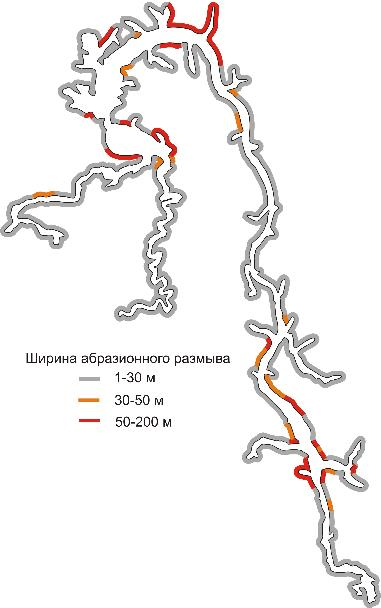
\includegraphics[width=\linewidth]{bratsk-reserv-shores.jpeg}
    \end{column}
    \begin{column}{0.6\linewidth}
      Результаты мониторинга: после более 50-ти лет эксплуатации  береговая зона все еще не достигла стадии устойчивого равновесия.  Сохраняется абразионный размыв, особенно береговых склонов, сложенных рыхлыми отложениями.

\vspace{1em}
От стабильности береговой зоны зависит возможность ее технического, рекреационного и др. видов использования, особенно в условиях, когда уровень воды регулируется технически в достаточно большом диапазоне значений сезонного (2-3 м) и многолетнего регулирования (до 10 м).
    \end{column}
  \end{columns}
\end{frame}


\begin{frame}[fragile]
  \frametitle{Береговая зона Братского водохранилища}
  \begin{columns}
    \begin{column}{0.5\linewidth}
      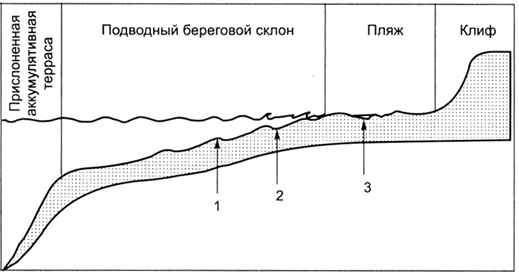
\includegraphics[width=\linewidth]{shore-struct-base.png}
      За положение береговой линии
принята последовательная линейная характеристика - положение бровки берегового уступа,  которое изменяется под воздействием волновой деятельности водохранилища и процессов разрушения берегового уступа.
    \end{column}
    \begin{column}{0.5\linewidth}
      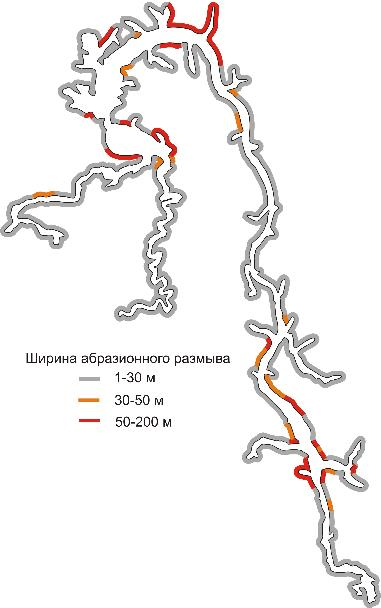
\includegraphics[width=\linewidth]{bratsk-reserv-shores.jpeg}
    \end{column}
  \end{columns}
\end{frame}

\begin{frame}[fragile]
  \frametitle{Прогнозирование конура береговой линии}
  \begin{columns}
    \begin{column}{0.6\linewidth}
      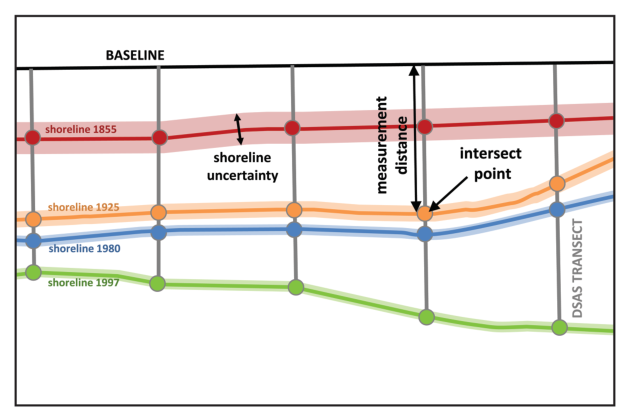
\includegraphics[width=\linewidth]{dsas-model.png}
    \end{column}
    \begin{column}{0.4\linewidth}
      Модель экстраполирует контур береговой линии по точкам вдоль нормали к базовой линии.  Исходными данными служат контуры береговых линий, соответствующие разным периодам времени.  Исходные данные для получение контуров -- спутниковые, аэрофотоснимки, съемка с квадрокоптера и топогеодезические данные.

      Проблема -- распознавание контуров береговых линий на растровых изображениях, имеющих различные характеристики.
    \end{column}
  \end{columns}
\end{frame}

\begin{frame}
  \frametitle{Технология SegmentAnything}
  \begin{columns}
    \begin{column}{0.25\linewidth}
      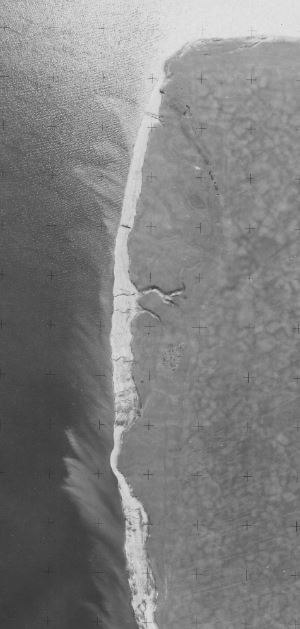
\includegraphics[width=1\linewidth]{photo-source.png}
    \end{column}
    \begin{column}{0.25\linewidth}
      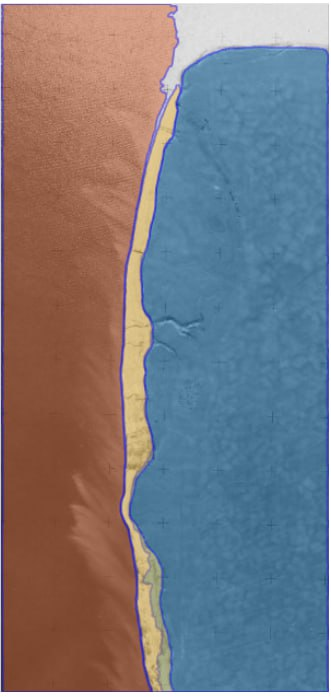
\includegraphics[width=1\linewidth]{sa-photo-result.png}
    \end{column}
    \begin{column}{0.25\linewidth}
      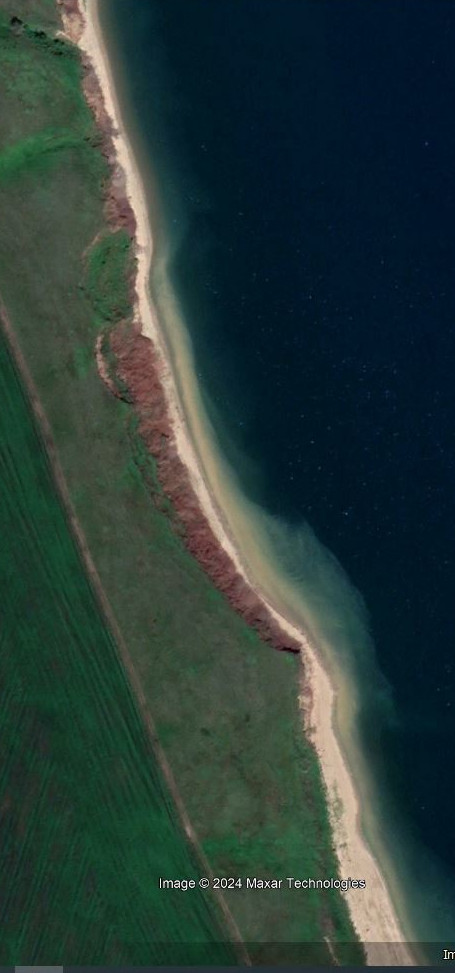
\includegraphics[width=1\linewidth]{source-img-ge.jpeg}
    \end{column}
    \begin{column}{0.25\linewidth}
      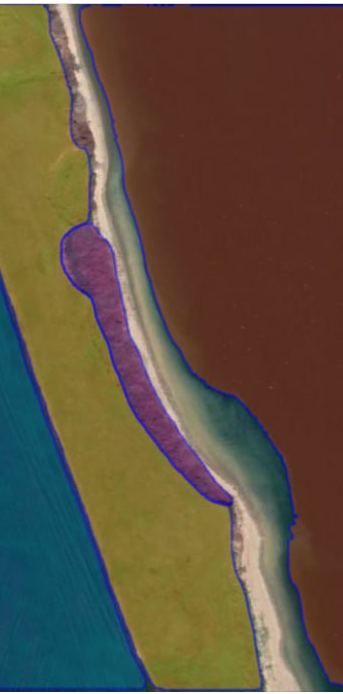
\includegraphics[width=1\linewidth]{sa-source-ge.png}
    \end{column}
  \end{columns}
  Техническая проблема -- на разнообразных цифровых изображениях распознать береговую линию:
  \begin{itemize}
  \item аэрофотоснимки,
  \item ортофотопланы,
  \item данные дистанционного зондирования Земли,
  \item топогеодезические съемки.
  \end{itemize}
\end{frame}

\begin{frame}
  \frametitle{Привязка разметки OpenStreetMap к ключевым точкам}
  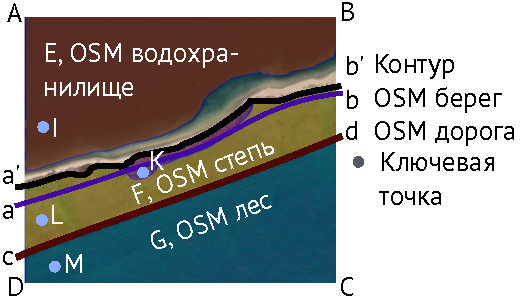
\includegraphics[width=1\linewidth]{tracing.pdf}
\end{frame}

\begin{frame}
  \frametitle{Архитектура распределенного сервиса}
  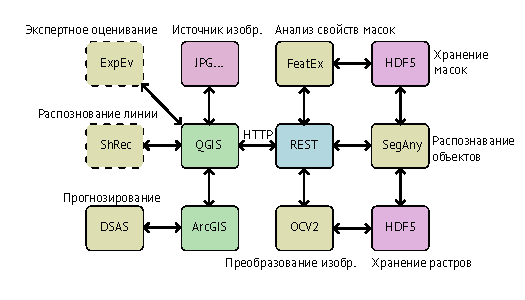
\includegraphics[width=1\linewidth]{arch.pdf}
\end{frame}

\begin{frame}
  \frametitle{Технология}
  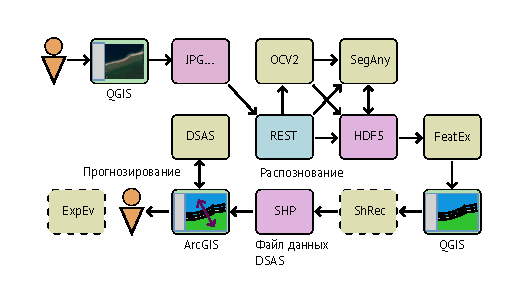
\includegraphics[width=1\linewidth]{tech.pdf}
\end{frame}

\begin{frame}
  \frametitle{Интерфейс ГИС со средой обработки информации}
  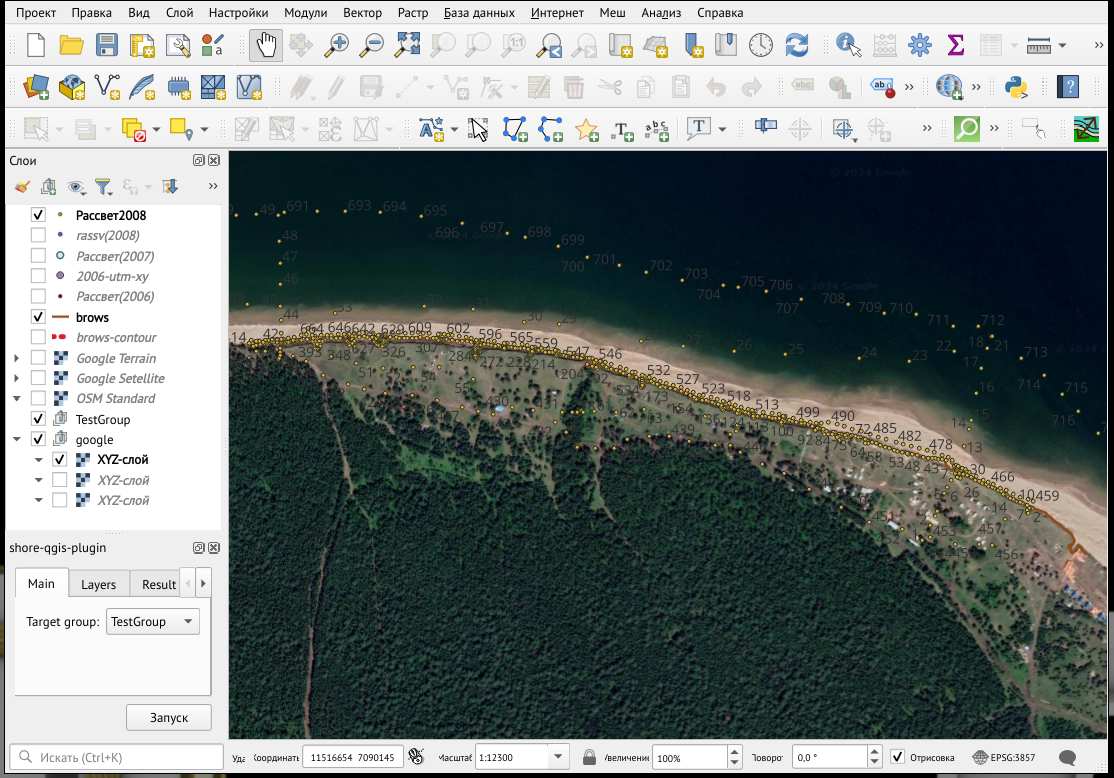
\includegraphics[width=1\linewidth]{screen-qgis.png}
\end{frame}

\begin{frame}
  \frametitle{Заключение по первому приложению}
  Сервис реализован примерно на 30\%, из оставшегося 30\% -- решение задачи распознавания береговой линии, остальное -- реализация технических задач.
  \begin{enumerate}
  \item SegmentAnything достаточно универсален и независим от свойств входного изображения
    \begin{itemize}
    \item наличие цветности,
    \item разрешения,
    \item размера,
    \end{itemize}
  \item Нет необходимости тратить время на подготовку изображений для качественного обучения
  \item Решение задачи распознавания вовлекает свободно сторонние ресурсы
  \item Верификация результатов распознавания НС в контексте логической задачи (теории)
  \end{enumerate}
  Дальнейшие направления совершенствования сервиса --
  \begin{enumerate}
  \item генерация данных для обучения НС,
  \item разработать итеративный алгоритм последовательного уточнения контура -- переходить к изображениям высокого разрешения на следующем шаге.
  \end{enumerate}
\end{frame}

\begin{frame}[fragile]
  \frametitle{Интерпретация как трансформация. Model--Driven Architecture}
  \begin{columns}
    \begin{column}{0.4\textwidth}
      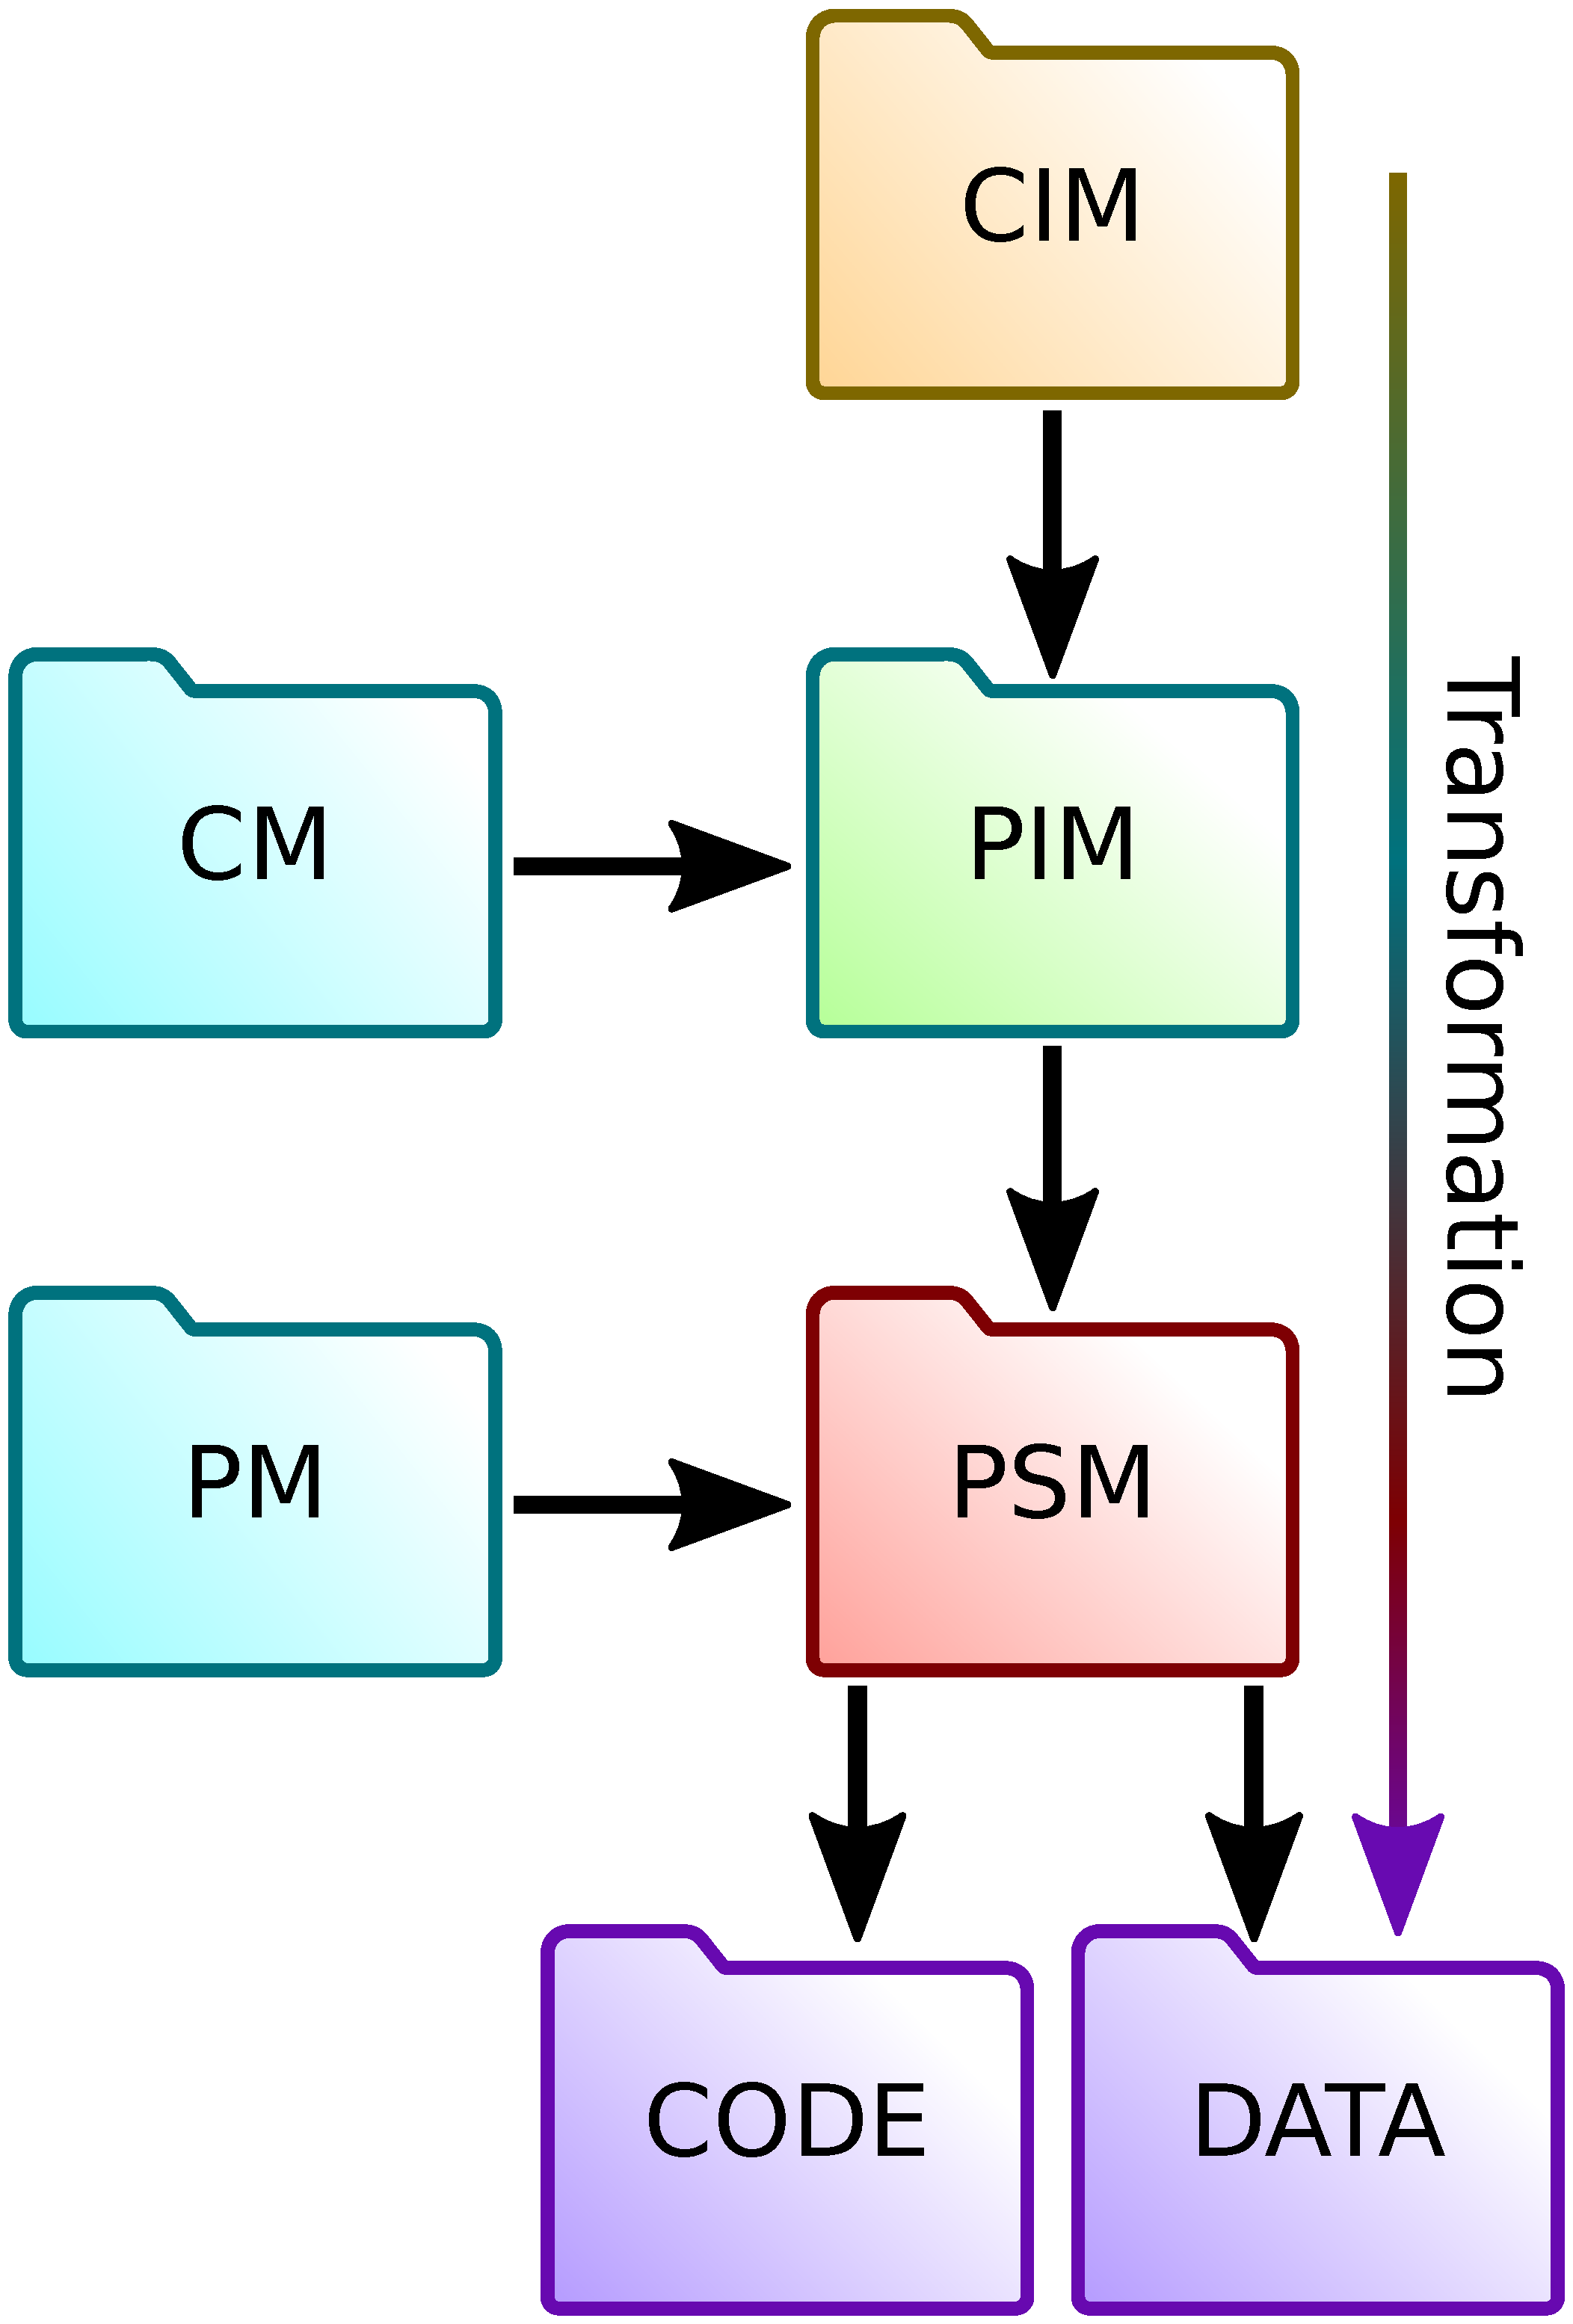
\includegraphics[width=1\linewidth]{mda-most-general.pdf}
    \end{column}
    \begin{column}{0.7\linewidth}
      \begin{description}
      \item[MDA] Model--Driven Architecture
      \item[CIM] Computationally Independent Model
      \item[CM] Model of Computations
      \item[PIM] Platform Independent Model
      \item[PM] Platform Model
      \item[PSM] Platform--Specific Model
      \item[CODE] Генерируемый исходный код
      \item[DATA] Начальное состояние баз данных
      \end{description}
    \end{column}
  \end{columns}
\end{frame}

\begin{frame}
  \frametitle{НИРОКР Model--Driven Architecture}
  \textbf{Основная цель} НИРОКР разработать технологии MDA, где модели CIM, PIM представлены в языках SysML, UML, BPMN, CMMN с использованием Семантического веба:
  \begin{enumerate}
  \item CIM представляется в UML, SysML, BPMN, CMMN, или как результат анализа текстов программ,
  \item PIM, PSM представляется в UML и в RDF с использованием стандартных онтологий,
  \item трансформации реализуются в языке Logtalk,
  \item сервера LOD запрашиваются на предмет дополнительной информации,
  \item порождение документов и интерфейсов пользователя, размеченных по требованиям LOD.
  \end{enumerate}
\end{frame}

% \begin{frame}
%   \frametitle{Related technologies and standards}
%   \begin{itemize}
%   \item The most widely used technologies \textbf{ATL} and its predecessor QVT, an OMG standard; developed for XMI to XMI conversion;
%   \item Usage of ATL trending to shift to CIM level, \emph{e.g.}, BPMN diagram is converted into set of UML diagrams (PIM); used for construction web-applications, CIM is represented with State and Use case UML-Diagrams.
%   \item MDA usage is widening, \emph{e.g.}, for analysis of security aspects of distributed application with logical inference over MDA represented model;
%   \item UML is used as CIM/PIM in modeling vocabularies (ontologies); there is an OMG standard specification;
%   \item XML specifications are used to describe services, \emph{e.g.} WSDL, WS-BPEL;
%   \item MDA is opposed to conceptual programming by Enn Tyugu.
%   \end{itemize}

%   We describe transformation in Logtalk, representing CIM, PIM and PSM as RDF graphs, allowing non-XMI sources to be used, organizing multi-stage modular transformations.
% \end{frame}

\begin{frame}[fragile]
  \frametitle{Технологии семантического веба -- элемент моделей трансформации}
  \begin{itemize}
  \item Использование результатов исследований, формализации и стандартизации предметных областей
  \item Граф знаний задается множеством троек
  \item Онтологии описываются формально (\verb|rdfs:domain|, \verb|rdfs:range|);
  \item Поддержаны в большинстве систем программирования библиотеками, механизмами логического вывода, SPARQL
  \item Существует способ глобальной идентификации объектов в RDF: в разных программах можно идентифицировать один о тот же объект
  \item SWI-Prolog поддерживает механизмы прямых запросов к графу и интерпретацию некоторых отношений (\verb|rdfs:label|, \verb|dc:title|)
  \item Простая поддержка разделения доступа к информации (\verb|rdfs:seeAlso|)
  \item Семантический веб и LOD -- основа интеграции приложений
  \end{itemize}
\end{frame}

\begin{frame}
\frametitle{Связанные открытые данные, LOD}
\begin{enumerate}
\item  Информация публикуется в Интернете с лицензией открытого доступа
\item  Он представлен в машиночитаемой форме, например, таблица Excel вместо растрового изображения
\item  открытый формат, используемый, например, CSV вместо Excel
\item  Формат основан на рекомендуемых стандартах W3C, что позволяет ссылаться на RDF и SPARQL
\item Опубликованные данные относятся к объектам, образующим контекст
\end{enumerate}
Таким образом, приложения публикуют данные как отношения объектов (сущностей).
\end{frame}


\begin{frame}
  \frametitle{Model Driven Architecture and Linked Open Data}
  \begin{center}
    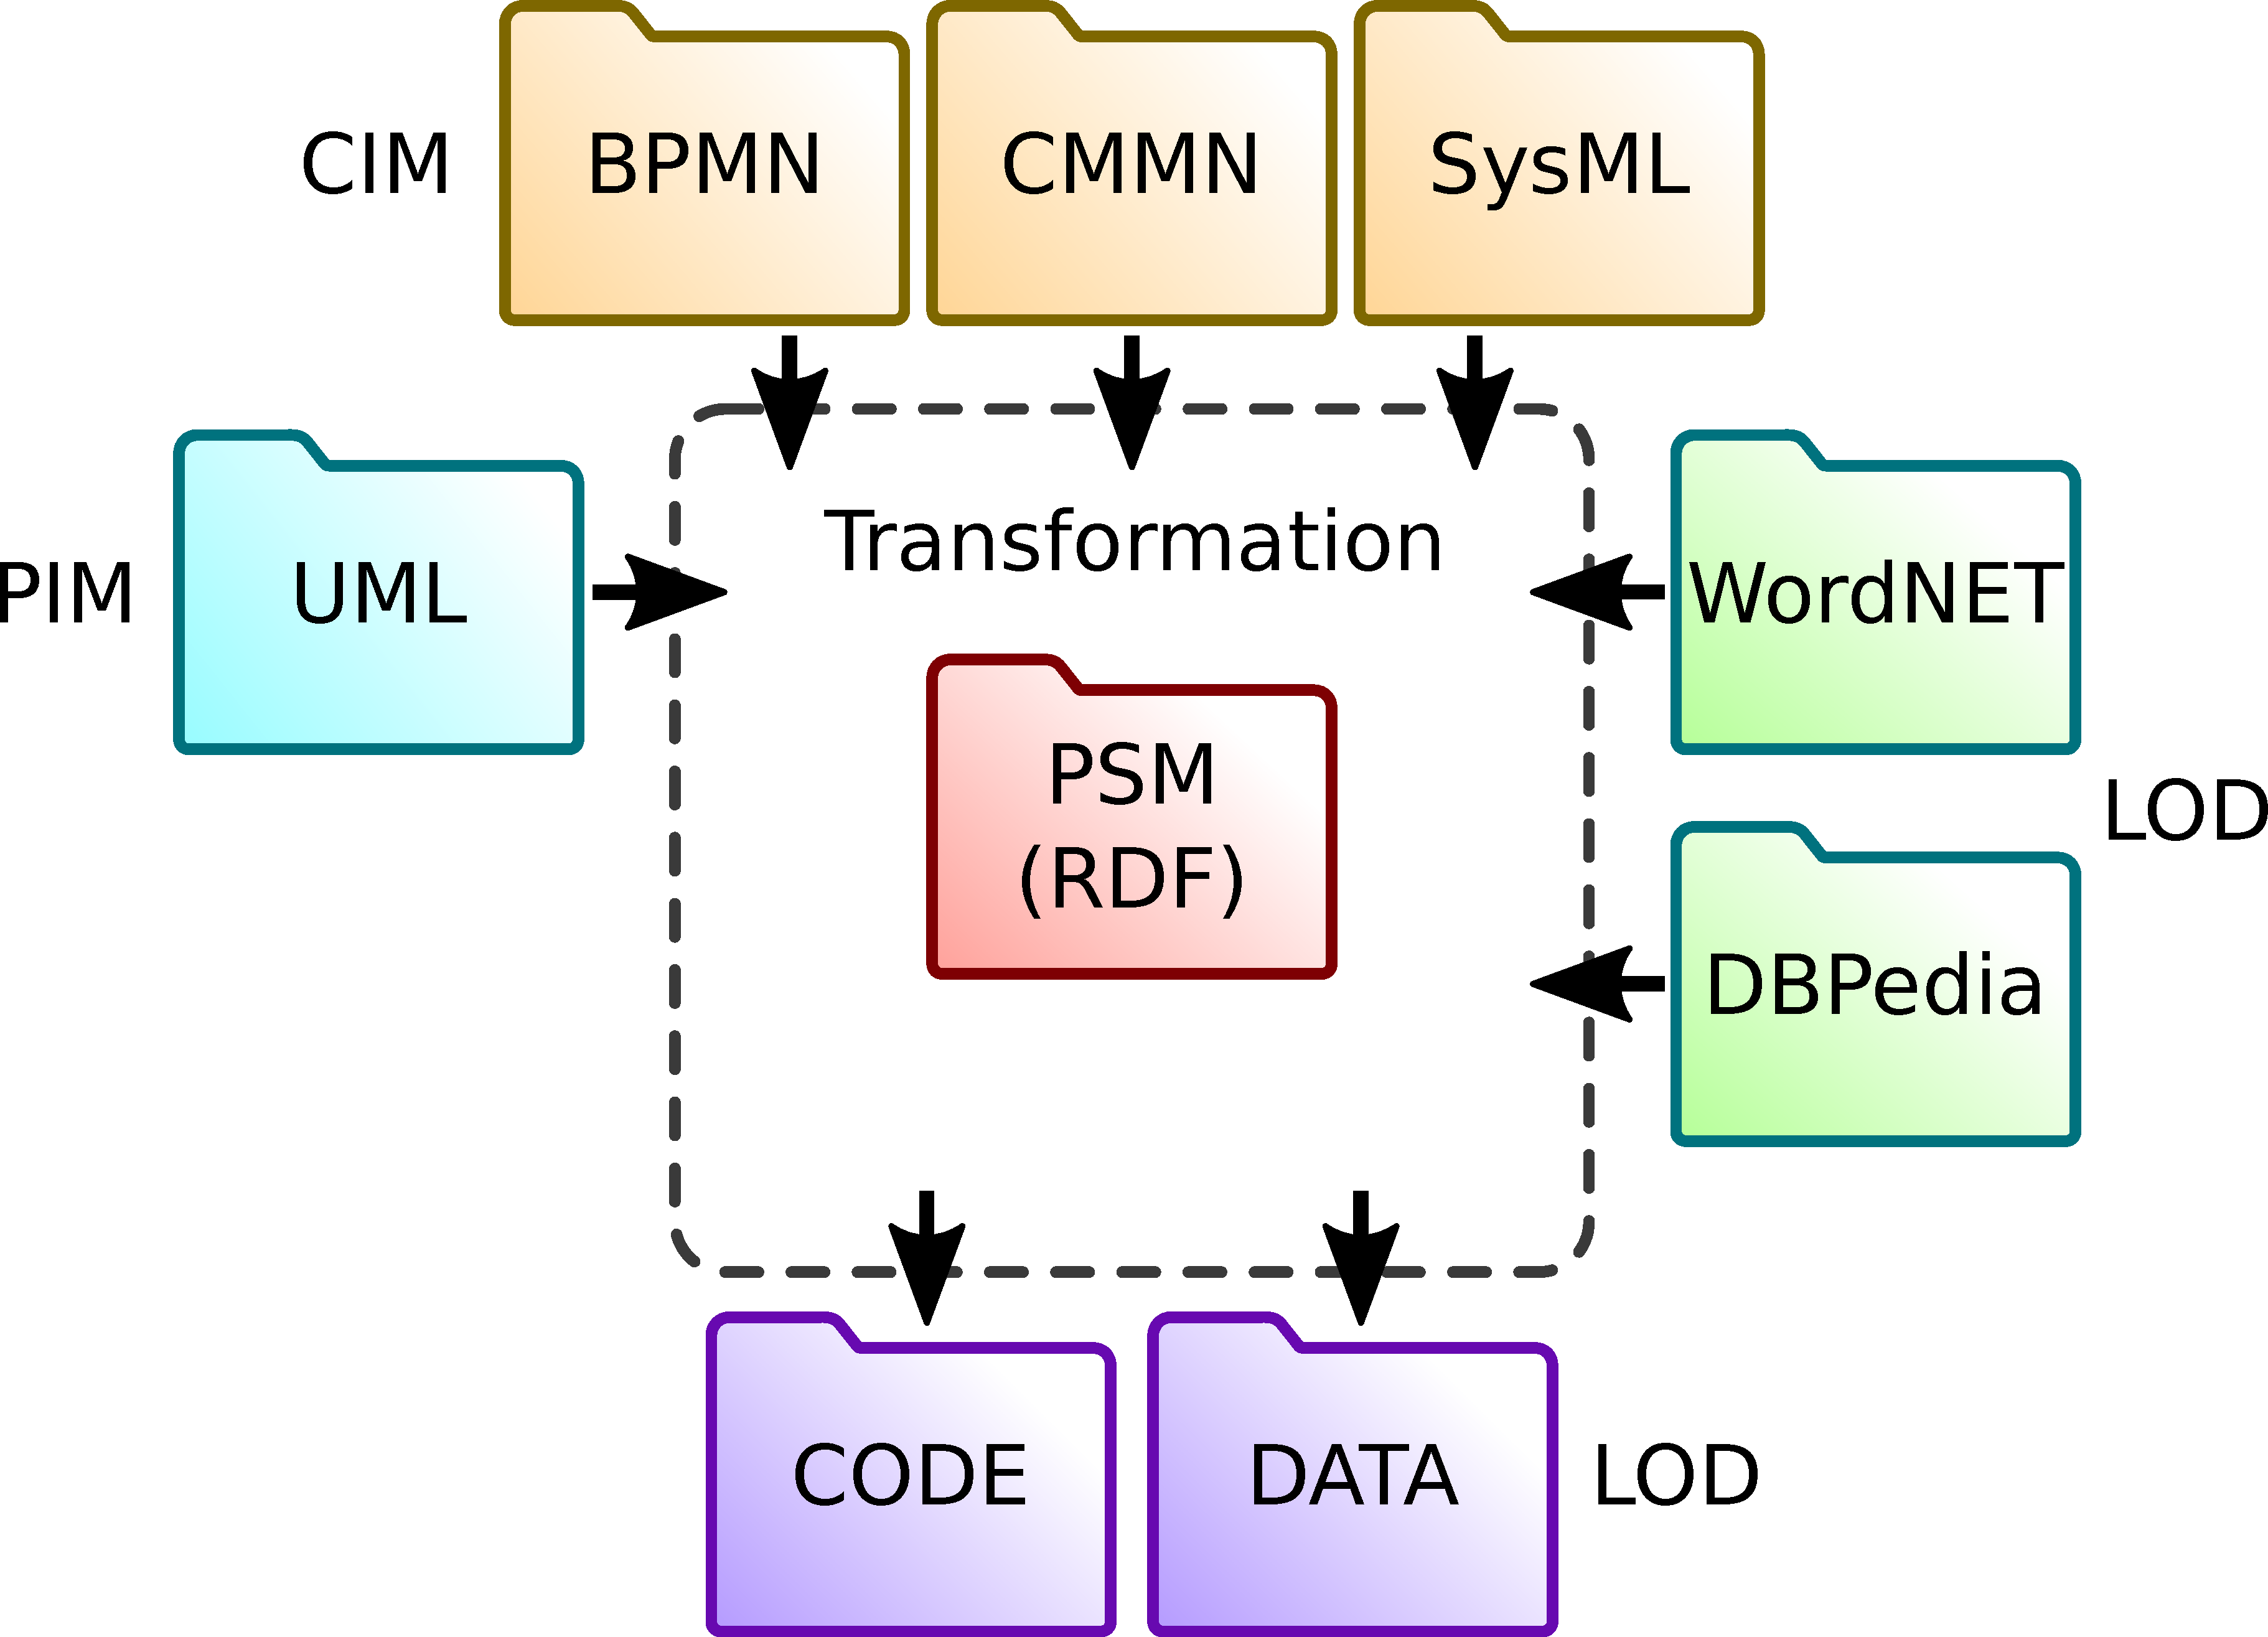
\includegraphics[width=0.9\linewidth]{mda-overview.pdf}
  \end{center}
\end{frame}

\begin{frame}
  \frametitle{Инфраструктура MDA}
  \centering
  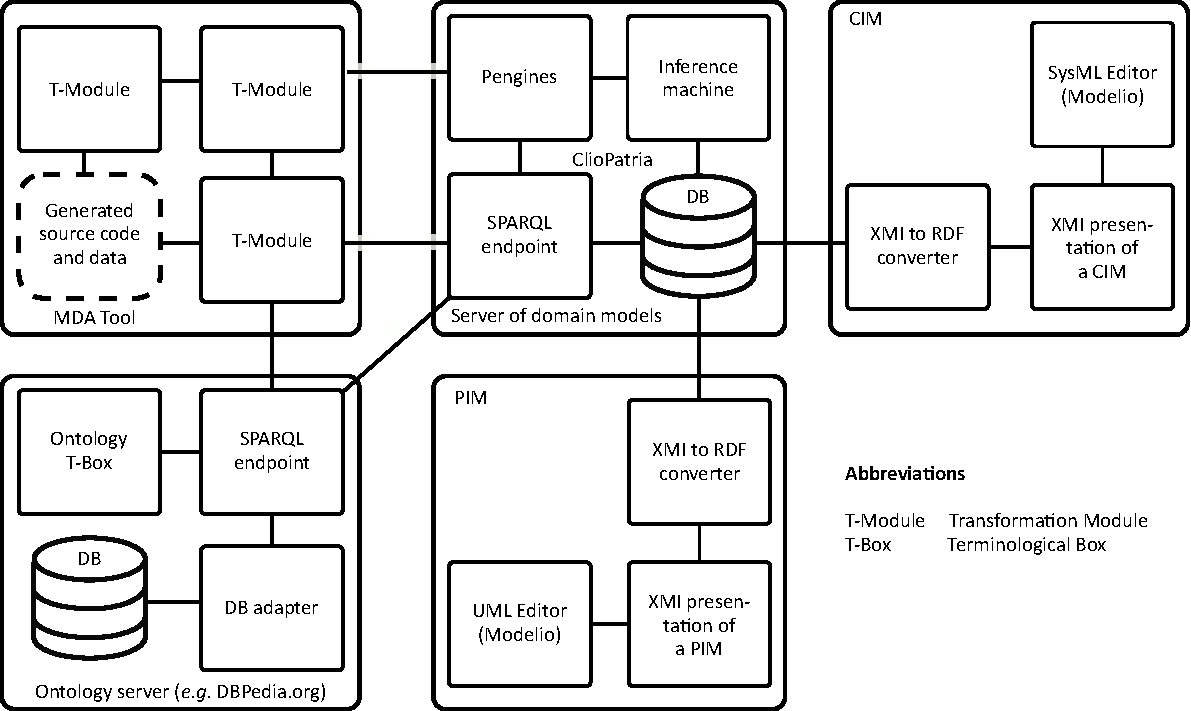
\includegraphics[width=1\linewidth]{architecture-mda-lod-ext.pdf}
\end{frame}

\begin{frame}
  \frametitle{Процесс трансформации}
  \centering
  % 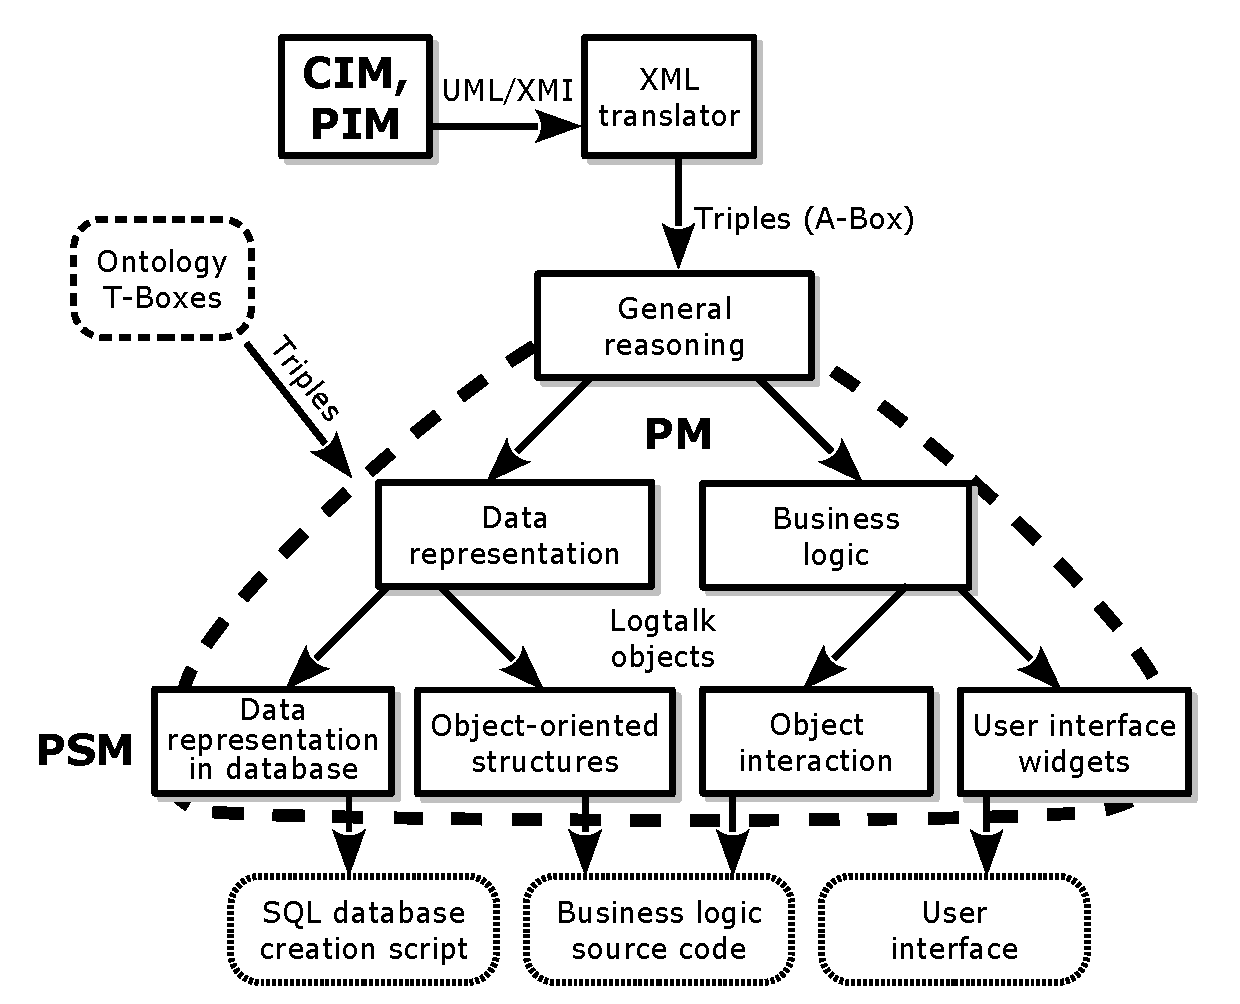
\includegraphics[width=0.9\linewidth]{architect_tree_pres-en-wo-OCL.pdf}
  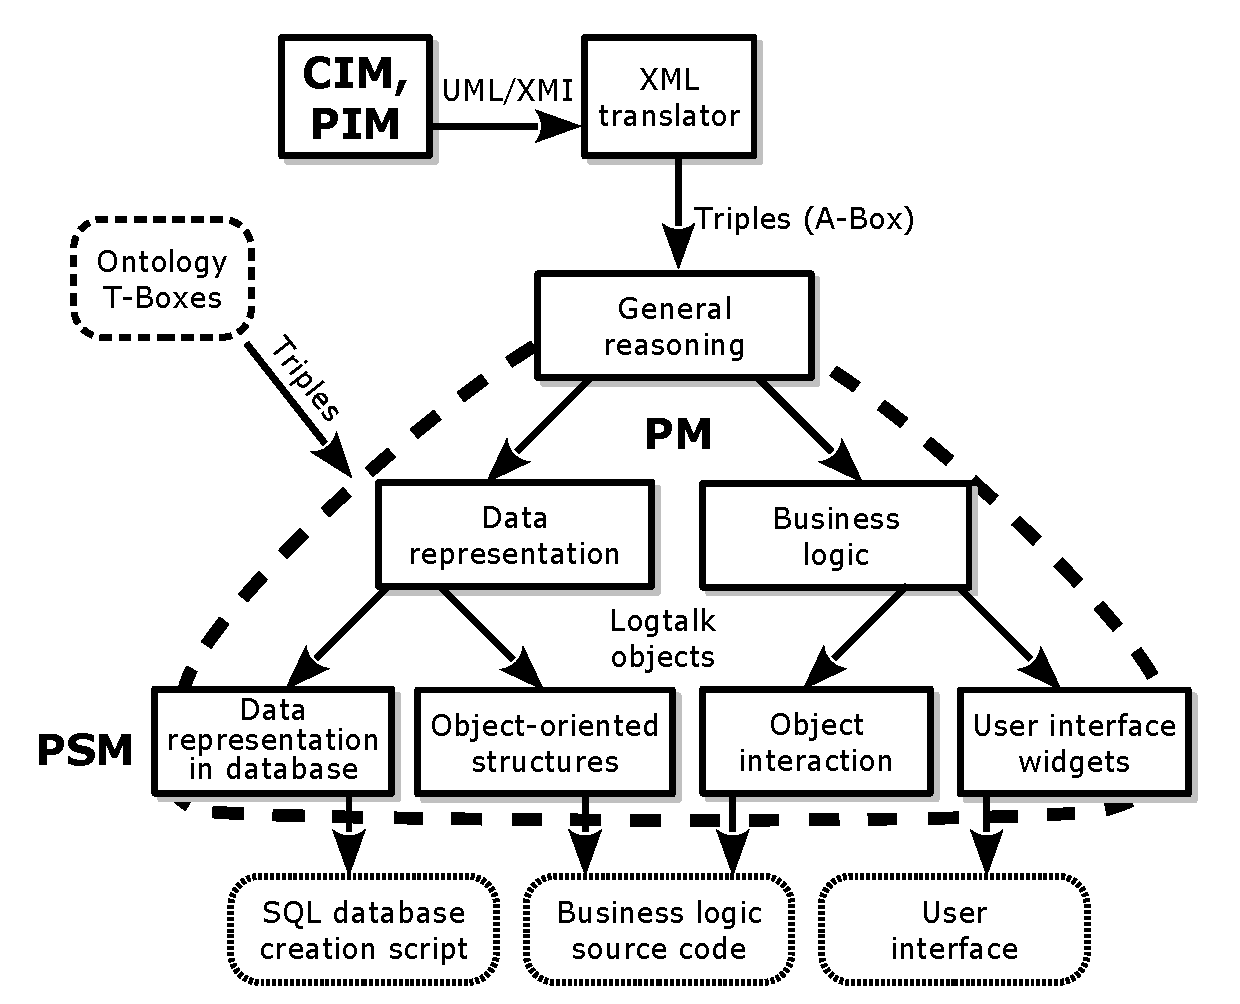
\includegraphics[width=0.9\linewidth]{architect_tree_pres-en-wo-OCL.pdf}
\end{frame}

\begin{frame}
  \frametitle{Logtalk -- средство манипуляции знаниями}
 % \frametitle{Logtalk as transformation definition language}
  Выбран, т.к. имеет следующие свойства:
  \begin{itemize}
  \item наследует широко известный синтаксис и среду исполнения Prolog
  \item реализован как макропакет, потери производительности составляют около 1.5-10\%
  \item имеет гибкую семантику: преобразования и ограничения определяются в рамках одного и того же синтаксиса
  \item реализует объектно-ориентированное структурирование знаний (правил), инкапсуляцию и замену
  \item из преобразований можно строить композиции
  \item механизм включения ограничений перехватом сообщений объекта к объекту (событий)
  \item есть варианты для различных реализаций ISO Prolog
  \end{itemize}
\end{frame}

\begin{frame}[fragile]
  \frametitle{Сценарий синтеза PSM}

%\begin{multicols}{2}
  \begin{columns}
    \begin{column}{0.6\textwidth}
\begin{minted}[fontsize=\tiny]{logtalk}
:- object(direct(_Package,_LocalProf,_CodeProf)).    % Transformation driver object
:- public([tr/4,tr/3]).                              % Public interface of a class synthesis scenario
% . . . . . . . . . .
tr(class, Class, ClassID):- ::package(Package),      % Synthesize a class
    query(Package)::class(Name, ClassID),            % Query package structure in XMI
    create_object(Class,      % . . . . .            % Create a <<Class>> object
    create_object(Attributes, % . . . . .            % Create <<Attributes>> object
    create_object(Methods,    % . . . . .            % ...<<Methods>>.
    Class::name(Name),                               % Name the class.
    % Generate attributes of the class,
    % organizing them in a local database.
    % ...methods...
    Class::attributes(Attributes),                   % Set the attributes for class.
    Class::methods(Methods).                         % ...methods.

tr(attribute, Attribute, ClassID, AttributeID):-     % Attribute transformations
    ::package(Package),
    query(Package)::attribute(Name,ClassID,AttrID),
    create_object(Attribute,  % . . . . .
    Attribute::name(Name).                           % Name the attribute.

tr(method, Method, ClassID, MethodID):-              % Transformation of methods
    ::package(Package),
    query(Package)::method(Name,ClassID,MethodID),
    create_object(Method,     % . . . . .
    Method::name(Name).                              % Name of the method
:- end_object.
\end{minted}
    \end{column}
    \begin{column}{0.4\linewidth}
      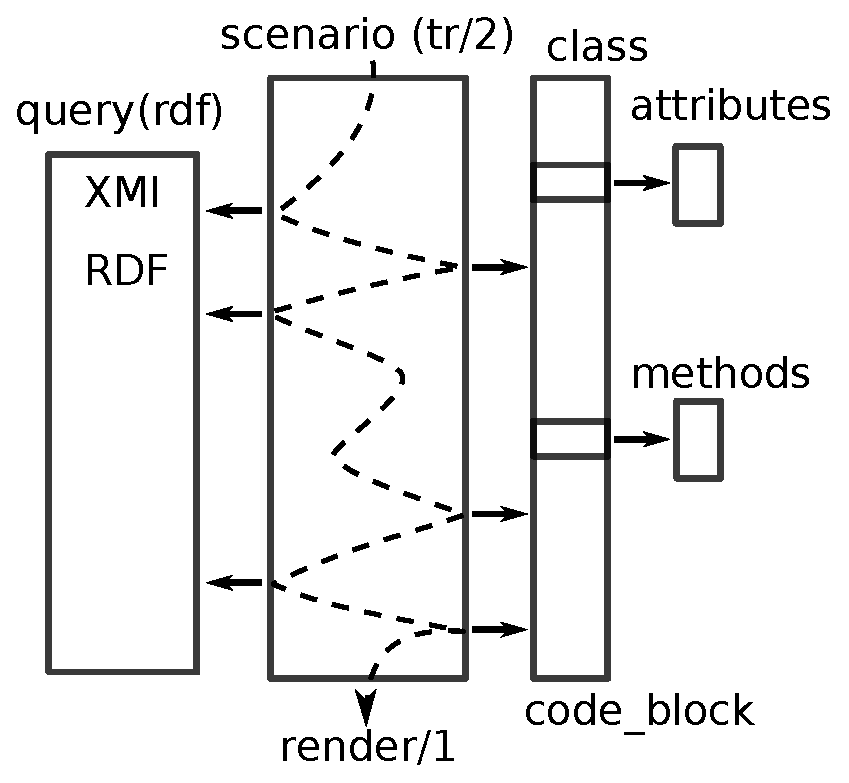
\includegraphics[width=1\linewidth]{scenario.pdf}
    \end{column}
  \end{columns}
  % \end{multicols}
\end{frame}

\begin{frame}[fragile]
  \frametitle{Обрамление модели PSM}
\begin{minted}[fontsize=\footnotesize{}]{logtalk}
:- object(query(_XMI)).
:- protected(xmi/1).
:- public([class/2, attribute/3, method/3]).
xmi(XMI) :- parameter(1, XMI).
class(Name, ID):-                            % Recognition of Class in RDF
    ::xmi(XMI),
    XMI::rdf(ID,rdf:type,uml:'Class'),
    XMI::rdf(ID,rdfs:label, literal(Name)).
attribute(Name, ClassID, ID):-               % ...attribute...
    ::xmi(XMI),
    XMI::rdf(ClassID, xmi:ownedAttribute, ID),
    XMI::rdf(ID, rdfs:label, literal(Name)).
method(Name, ClassID, ID):-                  % ...method...
    ::xmi(XMI),
    XMI::rdf(ClassID, xmi:ownedOperation, ID),
    XMI::rdf(ID, rdfs:label, literal(Name)).
% . . . . . . . . . . .
:- end_object.
\end{minted}
\end{frame}

\begin{frame}[fragile]
  \frametitle{Блок кода. Идея -- \texttt{llvmlite}${}^*$}
  \begin{columns}
    \begin{column}{0.6\textwidth}
      \flushleft
\begin{minted}[fontsize=\footnotesize{}]{logtalk}
:- object(code_block, specializes(root)).
% Public interface of the object
:- public([append/1, prepend/1, clear/0,
   render/1, render_to/1, remove/1,
   item/1, items/1]).
% Code block items
:- dynamic([item_/1]).
:- private([item_/1]).
% Methods specialized during inheritance
:- protected([renderitem/2, render_to/2]).
% . . . . . . . . . . . .
% Delegate rendering to object itself
renderitem(Object, String):-
    current_object(Object), !,
    Object::render(String).
% Convert a literal to its string
% representation
renderitem(literal(Item), String):-!,
    atom_string(Item, String).
% Just print the item (debugging).
renderitem(Item, String):-
    root::iswritef(String, '%q', [Item]).
:- end_object.
\end{minted}
    \end{column}
    \begin{column}{0.4\textwidth}
      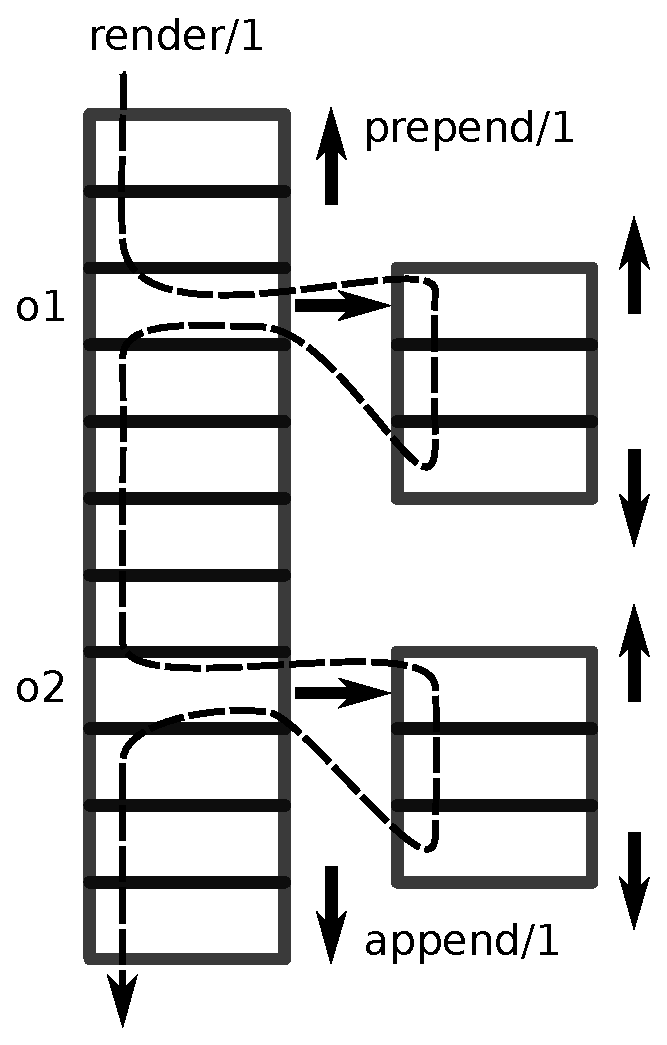
\includegraphics[width=1\linewidth]{code_block.pdf}
  ${}^*$) \url{https://github.com/numba/llvmlite}
    \end{column}
  \end{columns}
\end{frame}

\begin{frame}[fragile]
  \frametitle{PSM-модель класса Python -- специализация блока кода}
%\begin{multicols}{2}
  \begin{columns}
    \begin{column}{0.6\textwidth}
      \flushleft
\begin{minted}[fontsize=\scriptsize]{logtalk}
:- object(class, specializes(code_block),
   imports([named])). % Category of named entities
:- public([classlist/1, methods/1, attributes/1]).
% . . . . . . . . . . . . . .
renderitem(Item, Result):-      % proceed with default
    ^^renderitem(Item, Result). % rendering
render(Result):-         % Source generator
    ^^render(Name),      % implemented in a category
    ( ::item(classlist(List)) ->
     % . . . . . . . . . . .
        [Name]) ),
    ( ::item(attributes(Attributes))->
     % . . . . . . . . . . .
        [DefAttrList]),
      Attributes::items(InstanceAttrs),
      findall(S, ( % initialize attributes
         % . . . . . . . . .
         ), AttrAssigns),
        root::unindent,
        AttrList=[ConstructorDef|AttrAssigns];
         % . . . . . . . . .
        AttrList=[ConstructorDef, Pass] ),
    ( ::item(methods(Methods))-> % If any ...
      Methods::render(MethodList);
      MethodList=[] ),
    lists::append(AttrList,MethodList,StringList),
    root::unindent, Result=[Signature|StringList].
:- end_object.
\end{minted}
    \end{column}
    \begin{column}{0.4\linewidth}
      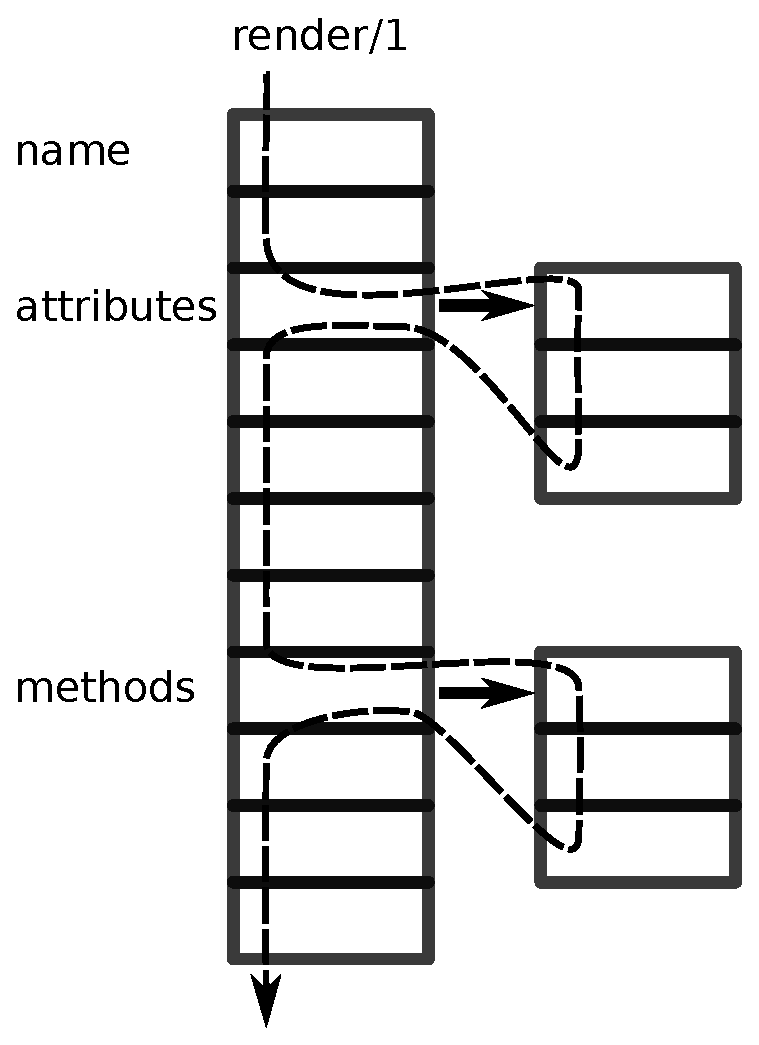
\includegraphics[width=1\linewidth]{code_block_class.pdf}
    \end{column}
  \end{columns}
  % \end{multicols}
\end{frame}

% \begin{frame}[fragile]
%   \frametitle{Logtalk Categories}
%   A category of named entities
% \begin{minted}[fontsize=\scriptsize]{logtalk}
% :- category(named).
% :- public([name/1, render/1]).
% :- protected([renderitem/2]).
% name(Name):- ::prepend(name(Name)).
% renderitem(name(Name), String):-!, atom_string(Name, String).
% render(String):-  % What is code generation from items
%     ::item(name(Name)), ::renderitem(name(Name), String).
% :-end_category.
% \end{minted}
% Category of named and typed entities
% \begin{minted}[fontsize=\scriptsize]{logtalk}
% :- category(namedtyped, extends(named)).
% :- public([type/1,render/2, separator_option/2,list_separator/1]).
% :- protected([renderitem/2]).
% type(Type):- ::append(type(Type)).
% renderitem(Item, String):- ^^renderitem(Item, String),!.
% renderitem(type(Type),String):-!, ::list_separator(Separator),
%     writef::swritef(String, '%w%w', [Separator, Type]).
% render(Middle, String):- ^^render(SName),
%     (   ::item(type(Type)) ->
%         ::renderitem(type(Type), SType),
%         string_concat(SName, Middle, _1),
%         string_concat(_1, SType, String) ;
%         SName = String  ).
% render(String):-  ::render("", String).
% list_separator(Separator):-
%     ::separator_option(Name, Default),!, % Global options
%     root::option(Name, Separator, Default).
% :- end_category.

% \end{minted}
% \end{frame}

\begin{frame}[fragile]
  \frametitle{Доступ к данным LOD}

  \begin{columns}
\begin{column}{0.5\textwidth}
\begin{minted}[fontsize=\scriptsize]{logtalk}
:- category(sparql).
:- public(query/2).
query(Pattern,Parameters,Row):-
    prepare(Pattern,Parameters,Query),
    server(Host,Port,Path),
    sparql_query(Query, Row,
        [host(Host),port(Port),path(Path)]).
:- protected(server/3).  % must be implemented
                         % by a subclass.
:- protected(prepare/3). % prepares a query
% . . . . . . . . . .    %             string.
:- end_category.

:- object(dbpedia, extends(sparql)).
:- protected(server/3).
server('dbpedia.org',80,'/sparql').
:- public(entity_name/2).
entity_name(Entity,Language,Name):-
    query('select ?name where { '
          ' %w rdfs:label ?name. '
          'FILTER langMatches( lang(?label),'
          ' "%w" )}', [Entity, Language],
          row(Name)).
:- end_object.

% ?- dbpedia::entity_name(dbr:'Passport', 'ru', Name).
\end{minted}
\end{column}
\begin{column}{0.5\textwidth}
  \flushright
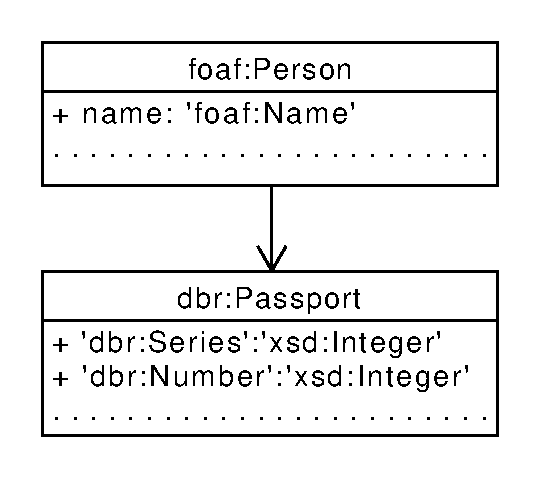
\includegraphics[width=0.8\linewidth]{simple-diag.pdf}
\end{column}
\end{columns}
\end{frame}


% \begin{frame}
%   \frametitle{Application in developing KBS}
%   Development and maintaining applied \textbf{knowledge--based systems (KBS)} in the up to date adequate state requires a lot of efforts devoted to solving problems of
%   \begin{itemize}
%   \item data model evolution,
%   \item functionality expansion,
%   \item graphical user interface modification.
% \end{itemize}

% To address these problems and, therefore, reduce the cost of creating, modifying and upgrading of applied KBS an automation of KBS development process is required.
% \end{frame}

% \begin{frame}
%   \frametitle{Application in developing KBS}
%   \begin{center}
%   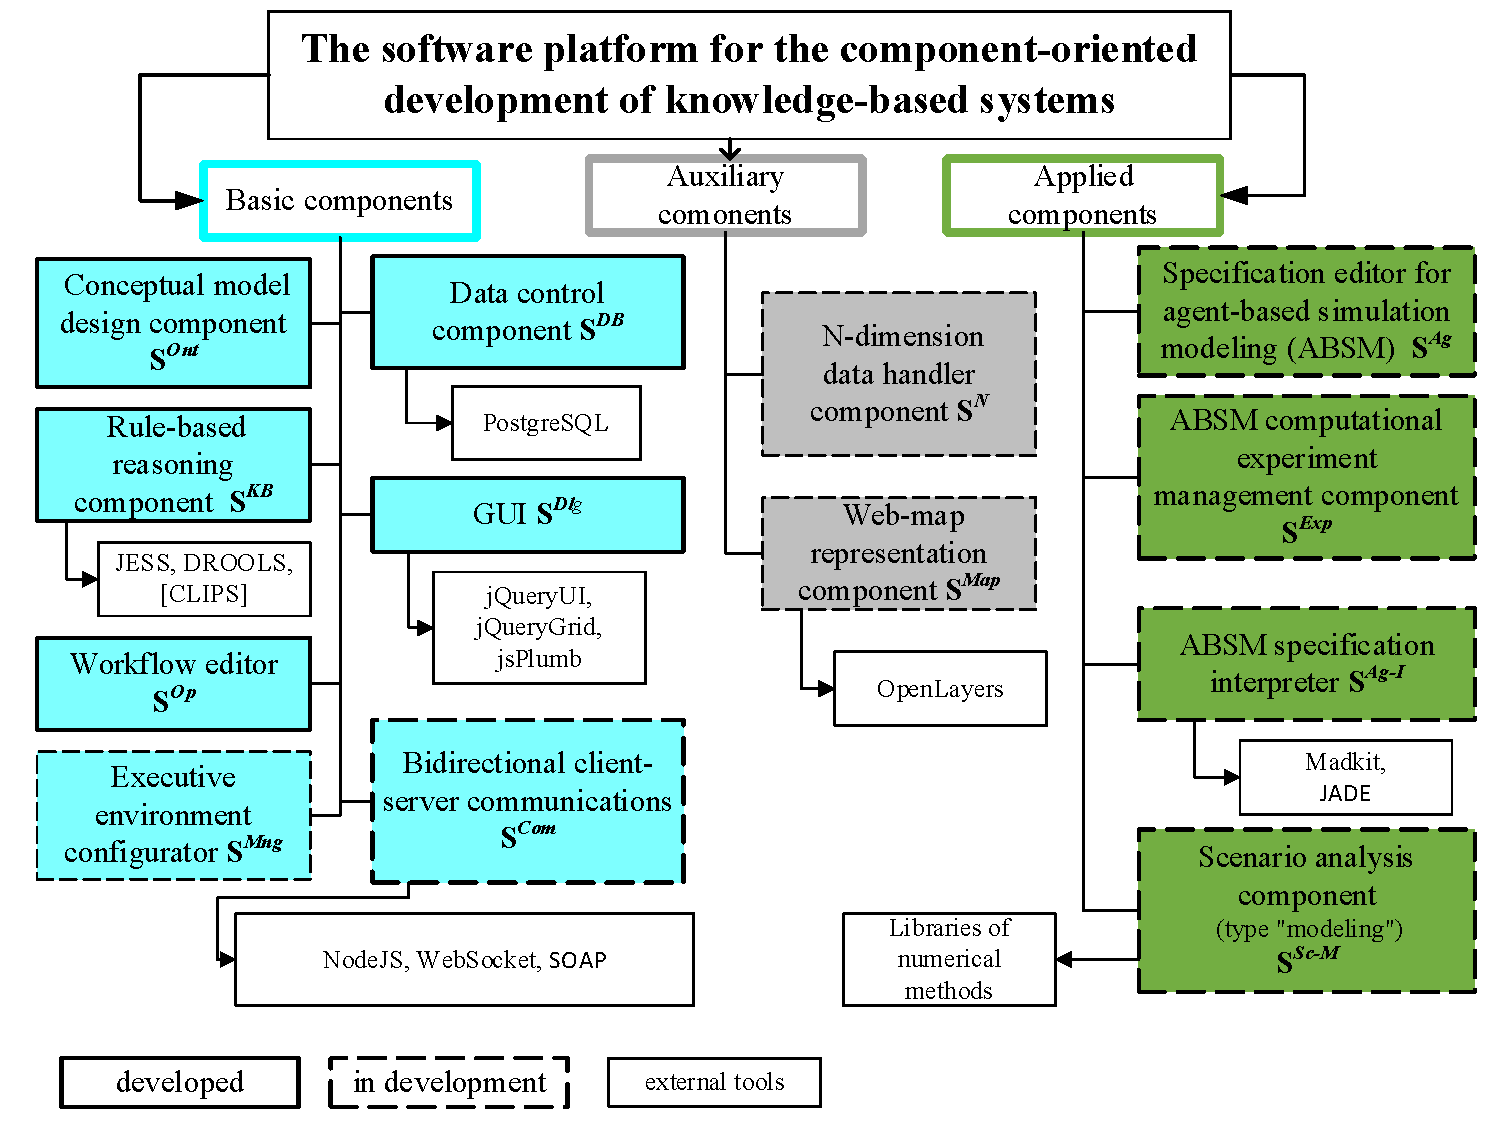
\includegraphics[width=0.9\linewidth]{kbs-stolboff.pdf}
% \end{center}
% \end{frame}

\begin{frame}[fragile]
  \frametitle{Модуль Rapidminer}
\begin{minted}[fontsize=\tiny]{cpp}
vector<string> AlignCommand::setParameters(){ // PART OF MODULE SOURCE
try {
  CommandParameter ptemplate("reference", "InputTypes", "", "", "none", "none", "none","",false,true,true); parameters.push_back(ptemplate);
  CommandParameter pcandidate("fasta", "InputTypes", "", "", "none", "none", "none","fasta-alignreport-accnos",false,true,true); parameters.push_back(pcandidate);
  CommandParameter psearch("search", "Multiple", "kmer-blast-suffix", "kmer", "", "", "","",false,false,true); parameters.push_back(psearch);
  CommandParameter pksize("ksize", "Number", "", "8", "", "", "","",false,false); parameters.push_back(pksize);
  CommandParameter pmatch("match", "Number", "", "1.0", "", "", "","",false,false); parameters.push_back(pmatch);
// . . . . . . .
\end{minted}
\begin{minted}[fontsize=\tiny]{java}
package com.rapidminer.ngs.operator; // GENERATED JAVA MODULE
// imports

class MothurChimeraCcodeOperator extends MothurGeneratedOperator {
  private InputPort fastaInPort = getInputPorts().createPort("fasta");
  private InputPort referenceInPort = getInputPorts().createPort("reference");
  private OutputPort chimeraOutPort = getOutputPorts().createPort("chimera");
  private OutputPort mapinfoOutPort = getOutputPorts().createPort("mapinfo");
  private OutputPort accnosOutPort = getOutputPorts().createPort("accnos");

  public MothurChimeraCcodeOperator (OperatorDescription description) {
    super(description);
  }
  @Override
  public void doWork() throws OperatorException {
    super();
    // . . . . . .
  }
  @Override
  public List<ParameterType> getParameterTypes() {
    super();
        // . . . . . .
  }
  @Override
  public String getOutputPattern(String type) {
    if (type=="chimera") return "[filename],[tag],ccode.chimeras-[filename],ccode.chimeras";
    if (type=="mapinfo") return "[filename],mapinfo";
    if (type=="accnos") return "[filename],[tag],ccode.accnos-[filename],ccode.accnos";
    return super.getOutputPattern(type);
  }
}
\end{minted}
\end{frame}

\begin{frame}[fragile]
  \frametitle{Приложение: Диаграммы потока исполнения в NGS}
  \begin{columns}
    \begin{column}{0.6\textwidth}
      \begin{raggedright}
        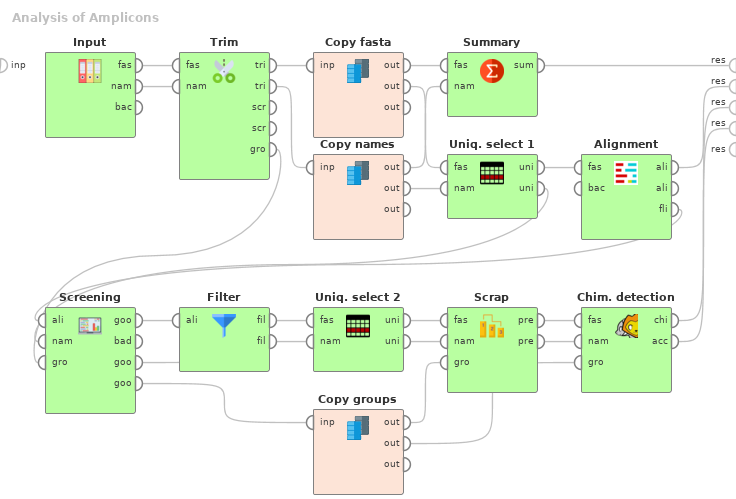
\includegraphics[width=1\linewidth]{Dataflow-color-en.png}
      \end{raggedright}
    \end{column}
    \begin{column}{0.4\textwidth}\footnotesize
      \begin{tabular}{ll}
        Термин & Расшифровка \\
        \hline
        NGS & New Generation \\
               & Sequencing \\
        Amplicon & часть ДНК, РНК, \\
               & скопированная \\
               & много раз \\
        Mothur & прикладной пакет \\
               & для NGS \\
        Rapidminer & визуальный \\
               & инструмент для \\
               & моделирования \\
               & процессов \\
               & Data Mining\\
               & и их исполнения
      \end{tabular}
      ${}$\\[1em]
      Зеленые блоки — это модули Mothur. Остальные -- модули Rapidminer.
    \end{column}
  \end{columns}
\end{frame}

\begin{frame}[fragile]
  \frametitle{Исхдоный граф RDF (TTL) и его обрамляющий объект}
\begin{multicols}{2}
\begin{minted}[fontsize=\tiny]{turtle}
@prefix xml: <http://www.w3.org/.../namespace> .
@prefix xsd: <http://www.w3.org/2001/XMLSchema#> .
ngsp:spec a ngsp:Specification ;
    ngsp:module mothur:NoCommand,
        mothur:align-check,
        mothur:align-seqs,
# . . . . .
mothur:align-check a ngsp:Module ;
    ngsp:outputPattern [ a cnt:Chars ;
            ngsp:parameterName "type" ;
            ngsp:pattern [ ngsp:patternString
                    "[filename],align.check" ;
                    dc:identifier "aligncheck" ] ;
            cnt:chars # . . . .
# . . . . .
mothur:align-check-idir-parameter
    a ngsp:Parameter ;
    ngsp:important false ;
    ngsp:multipleSelectionAllowed false ;
    ngsp:optionsDefault "" ;
    ngsp:required false ;
    ngsp:type mothur:String ;
    dc:title "inputdir" .

mothur:align-check-map-parameter a ngsp:Parameter ;
    ngsp:important true ;
    ngsp:multipleSelectionAllowed false ;
    ngsp:optionsDefault "" ;
    ngsp:required true ;
    ngsp:type mothur:InputTypes ;
    dc:title "map" .

mothur:align-check-name-parameter a ngsp:Parameter ;
    ngsp:chooseOnlyOneGroup "namecount" ;
    ngsp:important false ;
    ngsp:multipleSelectionAllowed false ;
# . . . . .
\end{minted}
\begin{minted}[fontsize=\tiny]{logtalk}
:- object(queryparam(_RDF,_Parameter),
          extends(ngsquerybase)).

:- public(type/1).
type(Type) :-
    ::attr(type, Type).
:- public(name/1).
name(Name) :- ::attr(dc:title, literal(Name)).
:- public(options/1).
options(Value):- ::attr(options, Value).
:- public(options_default/1).
options_default(Value):-
    ::attr(optionsDefault, Value).
% . . . . . . . .
:- public(multiple_selection_allowed/0).
multiple_selection_allowed:-
    ::bool_attr(multipleSelectionAllowed).
:- public(required/0).
required:-
    ::bool_attr(required).
:- public(important/0).
important:-
    ::bool_attr(important).
:- protected(attr/2).
attr(NS:Name, Value):-
    ::ngs(RDF),
    ::second(Parameter),
    rdf_db::rdf_global_object(Value, V),
    RDF::rdf(Parameter, NS:Name, V).
attr(Name, Value):-
    \+ Name=_:_,!,
    ::ngs(RDF),
    ::second(Parameter),
    rdf_db::rdf_global_id(Value, V),
    RDF::rdf(Parameter, ngsp:Name, V).
% . . . . .
\end{minted}
\end{multicols}
\end{frame}

\begin{frame}
  \frametitle{Обсуждение}
Интересные положительные впечатления:
\begin{itemize}
\item Logtalk и RDF являются гибкими, универсальными и удобными средствами реализации MDA.
\item Лучшие средства реализации -- инкапсцляция в предикаты Prolog и объекты Logtalk;
\item Не все свойства Logtalk исследованы: необходимо разработаны эффективные методики программирования, включая перехват сообщений.
\end{itemize}
Технические проблемы, затрудняющие использование Logtalk:
\begin{itemize}
\item Очень простые задачи требуют слишком много усилий, например, конвертация идентификатора в CamelCase.
\item Много времени уходит на изучение свойств существующих онтологий, но это более продуктивно, чем разработка <<с нуля>>;
\item Prolog не является популярным языком в MDA, как и Logtalk.
\end{itemize}
\end{frame}

% \begin{frame}
%   \frametitle{Еще польза для машинного обучения}
%   Тенденции развития систем ИИ
%   \begin{itemize}
%   \item Переход от рассуждений (логического вывода) к реакции по шаблонам
%   \end{itemize}
%   Реализация тенденций
%   \begin{itemize}
%   \item Использовать маски Segment Anything и результаты распознавания в качестве данных для обучения
%   \end{itemize}
% \end{frame}


\begin{frame}
  \frametitle{Заключение}
  К настоящему времени получены следующие результаты:
  \begin{itemize}
  \item Разработана и протестирована техника представления моделей
  \item Разработана методика программирования на объектно-ориентированном логическом языке Logtalk
  \item Реализованы прототипы различных операций трансформации
  \item Инструменты трансформации протестированы в прикладных областях, и никаких существенных технических проблем не было отмечено
  \end{itemize}
  Дальнейшие направления развития следующие:
  \begin{itemize}
  \item Техника для автоматической разметки документов при помощи сущностей онтологий
  \item Разработка методики реализации трансформации, минимизирующей использование динамических объектов и ориентированной на макро-возможности Logtalk
  \item Формирование набора инструментов из существующих прототипов, отвечающих современным требованиям разработки программного обеспечения
  \end{itemize}
  Исхдоный код проекта опубликован на Github:\\
\url{https://github.com/isu-enterprise/icc.xmitransform},\\ \url{https://github.com/eugeneai/icc.mothurpim}.
\end{frame}

% \begin{frame}
%    \frametitle{Вывод (заключительный)}
%    \begin{itemize}
%    \item Классические системы, основанные на знаниях, являются мощными инструментами ИИ для решения широкого класса задач распознавания и синтеза различного рода: исходного кода, объектов данных, управления
%    \item Современные средства сочетают в себе классические и новые подходы
%    \item Менее зависимы от вычислительных ресурсов (по сравнению с машинным обучением)
%    \item Позволяют обосновать полученные решения
%    \item Охватывают больший круг задач
%    \item Естественно для математических наук и требует более высокого уровня образования в области ИИ
%    \end{itemize}
%  \end{frame}


\begin{frame}
  \begin{center}
    \Large Спасибо за внимание!
%\vfill
%
\includegraphics[width=0.4\linewidth]{presentation.png}
%\url{https://github.com/eugeneai/talk-yantai-2023-12-18/blob/master/talk-la-in-soft-data-%design-2023-12-18.pdf}
\end{center}
\end{frame}

\end{document}

%%% Local Variables:
%%% mode: latex
%%% TeX-master: t
%%% End:
